\documentclass[xcolor=dvipsnames,serif]{beamer}\usepackage[]{graphicx}\usepackage[]{color}
%% maxwidth is the original width if it is less than linewidth
%% otherwise use linewidth (to make sure the graphics do not exceed the margin)
\makeatletter
\def\maxwidth{ %
  \ifdim\Gin@nat@width>\linewidth
    \linewidth
  \else
    \Gin@nat@width
  \fi
}
\makeatother

\definecolor{fgcolor}{rgb}{0.345, 0.345, 0.345}
\newcommand{\hlnum}[1]{\textcolor[rgb]{0.686,0.059,0.569}{#1}}%
\newcommand{\hlstr}[1]{\textcolor[rgb]{0.192,0.494,0.8}{#1}}%
\newcommand{\hlcom}[1]{\textcolor[rgb]{0.678,0.584,0.686}{\textit{#1}}}%
\newcommand{\hlopt}[1]{\textcolor[rgb]{0,0,0}{#1}}%
\newcommand{\hlstd}[1]{\textcolor[rgb]{0.345,0.345,0.345}{#1}}%
\newcommand{\hlkwa}[1]{\textcolor[rgb]{0.161,0.373,0.58}{\textbf{#1}}}%
\newcommand{\hlkwb}[1]{\textcolor[rgb]{0.69,0.353,0.396}{#1}}%
\newcommand{\hlkwc}[1]{\textcolor[rgb]{0.333,0.667,0.333}{#1}}%
\newcommand{\hlkwd}[1]{\textcolor[rgb]{0.737,0.353,0.396}{\textbf{#1}}}%
\let\hlipl\hlkwb

\usepackage{framed}
\makeatletter
\newenvironment{kframe}{%
 \def\at@end@of@kframe{}%
 \ifinner\ifhmode%
  \def\at@end@of@kframe{\end{minipage}}%
  \begin{minipage}{\columnwidth}%
 \fi\fi%
 \def\FrameCommand##1{\hskip\@totalleftmargin \hskip-\fboxsep
 \colorbox{shadecolor}{##1}\hskip-\fboxsep
     % There is no \\@totalrightmargin, so:
     \hskip-\linewidth \hskip-\@totalleftmargin \hskip\columnwidth}%
 \MakeFramed {\advance\hsize-\width
   \@totalleftmargin\z@ \linewidth\hsize
   \@setminipage}}%
 {\par\unskip\endMakeFramed%
 \at@end@of@kframe}
\makeatother

\definecolor{shadecolor}{rgb}{.97, .97, .97}
\definecolor{messagecolor}{rgb}{0, 0, 0}
\definecolor{warningcolor}{rgb}{1, 0, 1}
\definecolor{errorcolor}{rgb}{1, 0, 0}
\newenvironment{knitrout}{}{} % an empty environment to be redefined in TeX

\usepackage{alltt}
\usetheme{Boadilla}
\usecolortheme[named=CornflowerBlue]{structure}
\usepackage{graphicx}
\usepackage{breqn}
\usepackage{xcolor}
\usepackage{booktabs}
\usepackage{verbatim}
\usepackage{tikz}
\usepackage{lmodern}
\usetikzlibrary{shadows,arrows,positioning}
\definecolor{links}{HTML}{2A1B81}
\hypersetup{colorlinks,linkcolor=links,urlcolor=links}
\usepackage{pgfpages}

\tikzstyle{block} = [rectangle, draw, text width=9em, text centered, rounded corners, minimum height=3em, minimum width=7em, top color = white, bottom color=brown!30,  drop shadow]

% change font of frame titles and title slide
\setbeamerfont{title}{series=\bfseries}
\setbeamerfont{frametitle}{series=\bfseries} 

\newcommand{\ShowSexpr}[1]{\texttt{{\char`\\}Sexpr\{#1\}}}

\newcommand{\Bigtxt}[1]{\textbf{\textit{#1}}}
\IfFileExists{upquote.sty}{\usepackage{upquote}}{}
\begin{document}

\title[SWMPrats, Widgets]{The SWMPrats website and the Widgets}

\author[M. Beck]{Marcus W. Beck\inst{1}}

\date{}

\institute[]{\inst{1} USEPA NHEERL Gulf Ecology Division\\ Email: \href{mailto:beck.marcus@epa.gov}{beck.marcus@epa.gov}}

% knitr setup


% load SWMPr from local


%%%%%%
\begin{frame}
\vspace{0.3in}
\centerline{
\begin{tikzpicture}
  \node[drop shadow={shadow xshift=0ex,shadow yshift=0ex},fill=white,draw] at (0,0) {
\includegraphics[width=0.9\textwidth]{imgs/workshop2016logo.png}};
\end{tikzpicture}}
\titlepage
\end{frame}

\section{Overview}

%%%%%%
\begin{frame}{Objectives for the session (1:15 - 2:00)}
\begin{itemize}
\item Overview of the website \\~\\
\item Overview of the widgets \\~\\
\begin{itemize}
\item SWMP summary - evaluate trends of a single parameter at a single site \\~\\
\item SWMP trends - compare trends of a single parameter within and between reserves using a map \\~\\
\item SWMP aggregate - compare aggregated trends of different parameters within and between reserves \\~\\
\end{itemize}
\end{itemize}
\end{frame}

%%%%%%
\begin{frame}{Interactive portion}
\onslide<+->
We will use the widgets on the website or follow on my screen\\~\\
Following along as we go: \\~\\
\begin{itemize}
\item flash drive\\~\\
\item online: \href{http://swmprats.net/}{swmprats.net} 2016 workshop tab \\~\\
\end{itemize}
\onslide<+->
You will run examples whenever you see this guy: \\~\\
\centerline{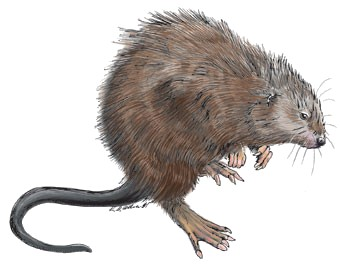
\includegraphics[width = 0.15\textwidth]{imgs/swmprat.png}} 
\end{frame}

\section{Overview}

%%%%%%
\begin{frame}{SWMPrats.net}
\centerline{\fbox{
\includegraphics[width = 0.95\textwidth]{imgs/swmprats_logo.png}}}
\vspace{0.2in}
\Large
\Bigtxt{S}ystem-\Bigtxt{W}ide \Bigtxt{M}onitoring \Bigtxt{P}rogram \\
\hspace{0.5in} \Bigtxt{R}esources for the \Bigtxt{A}nalysis of \Bigtxt{T}ime \Bigtxt{S}eries \\~\\
\normalsize
\end{frame}

%%%%%%
\begin{frame}{SWMPrats.net}
\begin{quote}
An ad hoc group formed to develop and expand the capacity of the NERRS program to more effectively use SWMP data 
\end{quote}
\vspace{0.2in}
1) Training workshops 2014, 2015, today \\~\\
\begin{columns}
\begin{column}{0.5\textwidth}
\centerline{\fbox{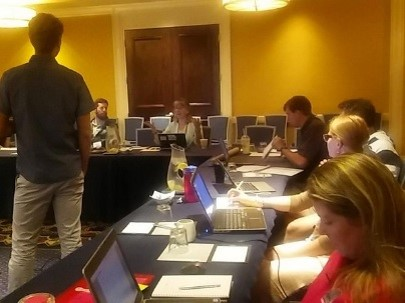
\includegraphics[width = 0.75\textwidth]{imgs/work1.jpg}}}
\end{column}
\begin{column}{0.5\textwidth}
\centerline{\fbox{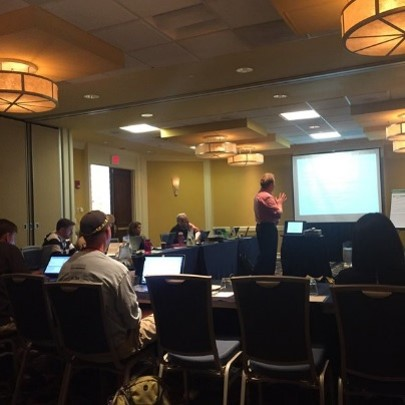
\includegraphics[width = 0.54\textwidth]{imgs/work2.jpg}}}
\end{column}
\end{columns}
\end{frame}

%%%%%%
\begin{frame}[fragile]{SWMPrats.net}
\centerline{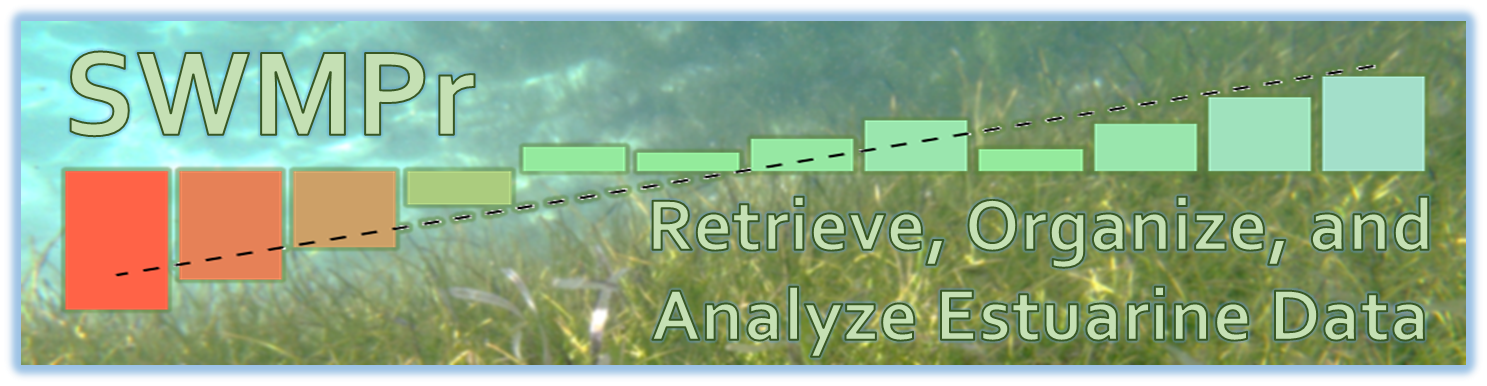
\includegraphics[width = 0.85\textwidth]{imgs/swmpr_logo.png}}
\vspace{0.2in}
2) SWMPr is an open-source R package described on the website, v2.1.7
\begin{knitrout}\scriptsize
\definecolor{shadecolor}{rgb}{0.969, 0.969, 0.969}\color{fgcolor}\begin{kframe}
\begin{alltt}
\hlcom{# install/load from R}
\hlkwd{install.packages}\hlstd{(}\hlstr{'SWMPr'}\hlstd{)}
\hlkwd{library}\hlstd{(SWMPR)}
\end{alltt}
\end{kframe}
\end{knitrout}
\end{frame}

%%%%%%
\begin{frame}{SWMPrats.net}
\centerline{\fbox{
\includegraphics[width = 0.75\textwidth]{imgs/swmprats_logo.png}}}
\vspace{0.15in}
3) \href{http://swmprats.net}{SWMPrats.net} (\#swmprats) is our base of operations... \\~\\
\begin{itemize}
\item Training materials \\~\\
\item SWMPr cookbook \\~\\
\item Forum (POTM)\\~\\
\item Widgets
\end{itemize}
\end{frame}

\section{Widgets}

%%%%%%
\begin{frame}{Widgets of SWMPrats.net}
Improved data integration and accessibility with a point-and-click approach \\~\\
Three Shiny applications allow users to visualize trends in SWMP data \\~\\
These apps allow `reactive' use of SWMPr functions \\~\\
\begin{columns}
\begin{column}{0.3\textwidth}
\centerline{\fbox{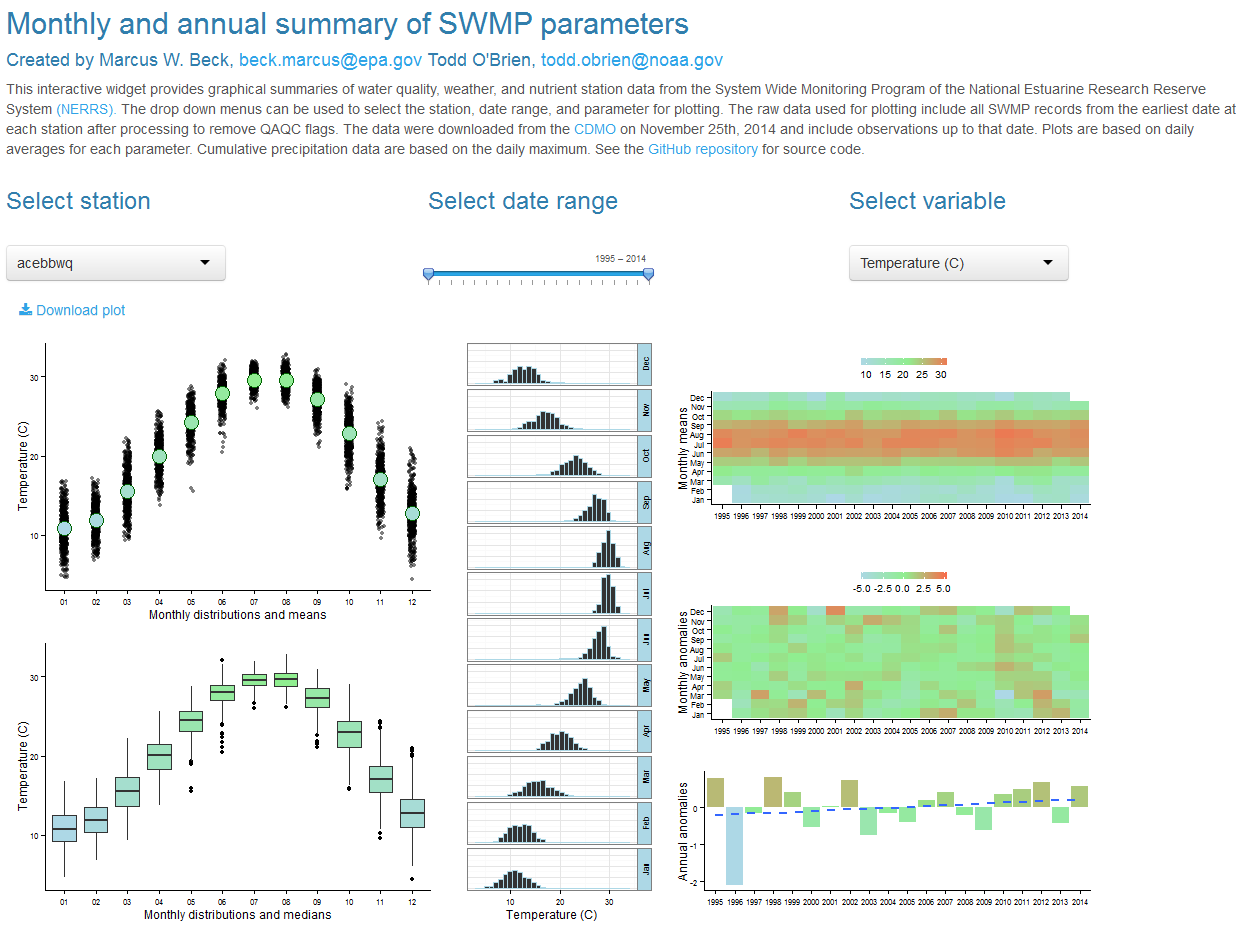
\includegraphics[width = 0.95\textwidth]{imgs/swmp_summary.png}}}
\end{column}
\begin{column}{0.3\textwidth}
\centerline{\fbox{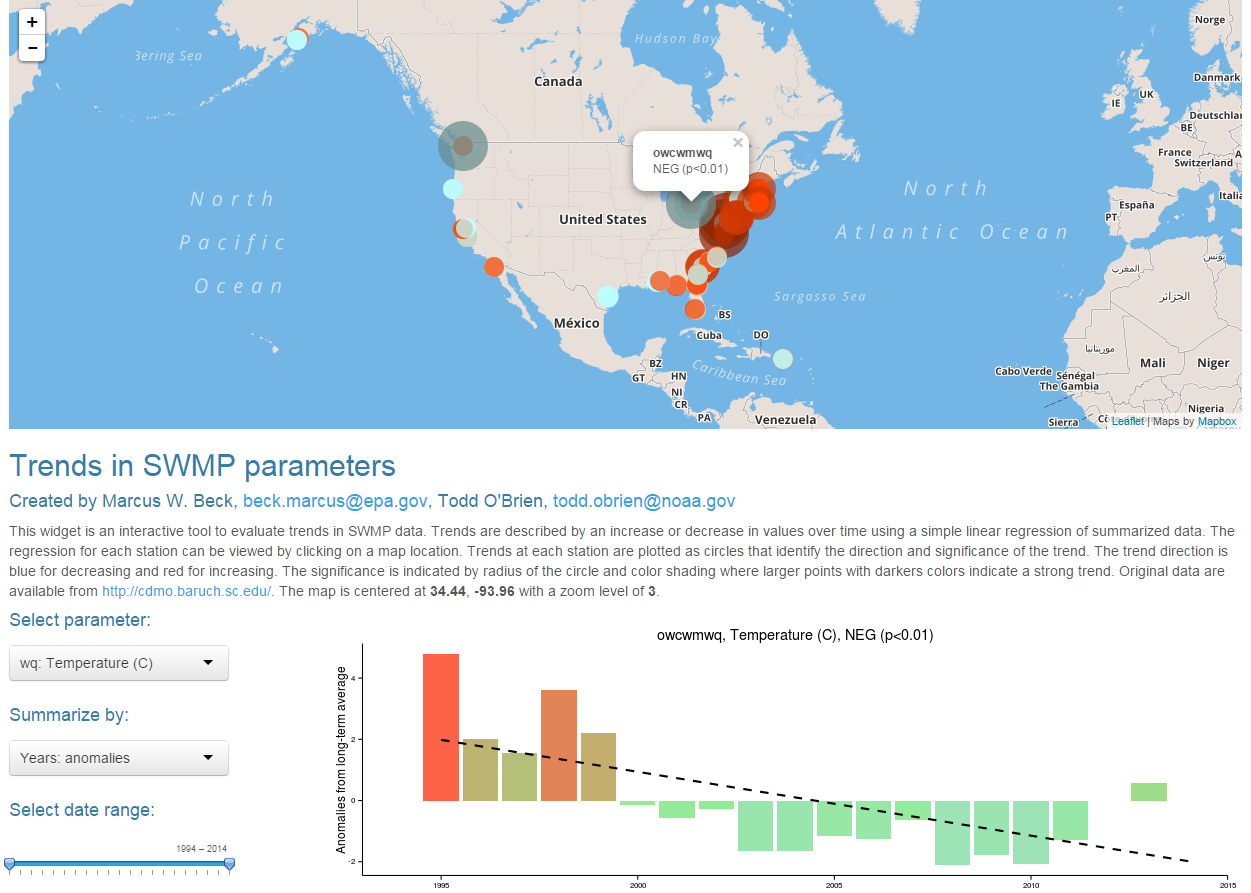
\includegraphics[width = 0.95\textwidth]{imgs/swmp_comp.png}}}
\end{column}
\begin{column}{0.3\textwidth}
\centerline{\fbox{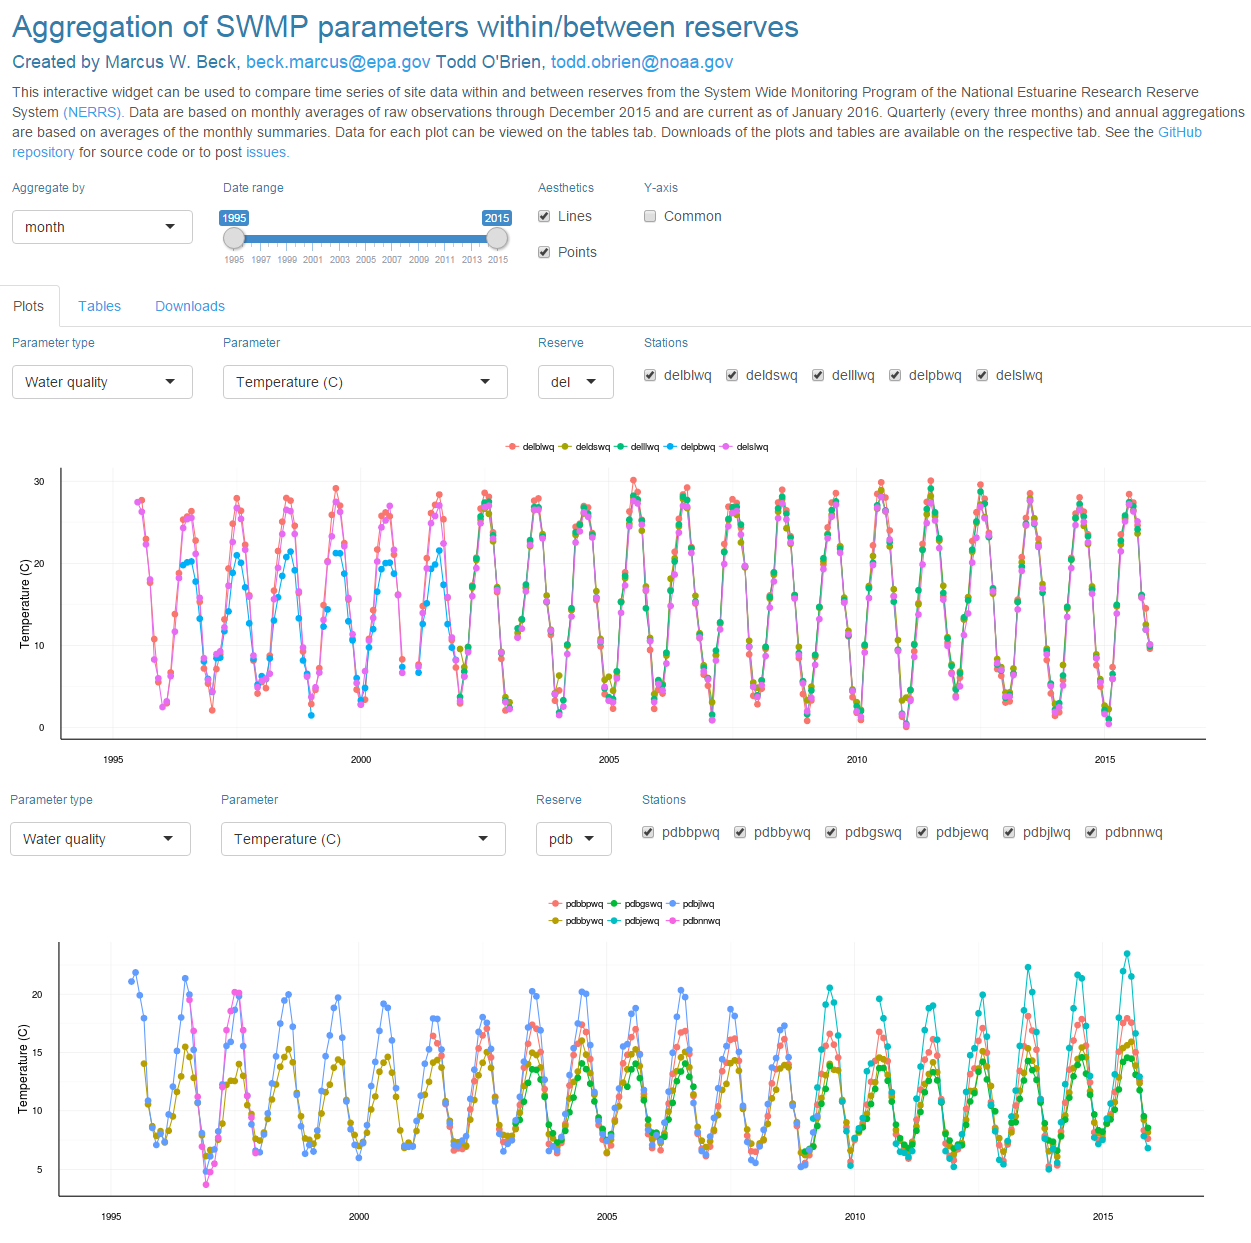
\includegraphics[width = 0.95\textwidth]{imgs/swmp_agg.png}}}
\end{column}
\end{columns}
\end{frame}

%%%%%%
\begin{frame}{Widgets of SWMPrats.net}
\onslide<1->
When using the widgets, understand... \\~\\
\begin{itemize}
\onslide<1->
\item Focus is on a single reserve or comparisons between reserves \\~\\
\onslide<2->
\item Focus is on a single parameter or comparisons between parameters \\~\\
\onslide<3->
\item They are for exploration - results or trends are not absolute \\~\\
\onslide<4->
\item Data have been processed a particular way - there are possible errors \\~\\
\onslide<5->
\item Data are static - hosted  directly with app or on private site after processing, updated once a year or catastrophic error...
\end{itemize}
\end{frame}

%%%%%%
\begin{frame}{Widgets of SWMPrats.net: SWMP summary}
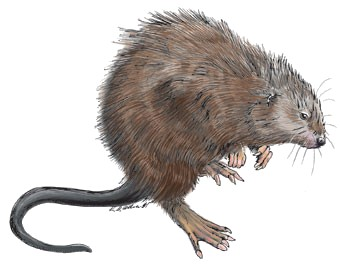
\includegraphics[width = 0.05\textwidth]{imgs/swmprat.png}  For summarizing trends at one site and one parameter
\centerline{\fbox{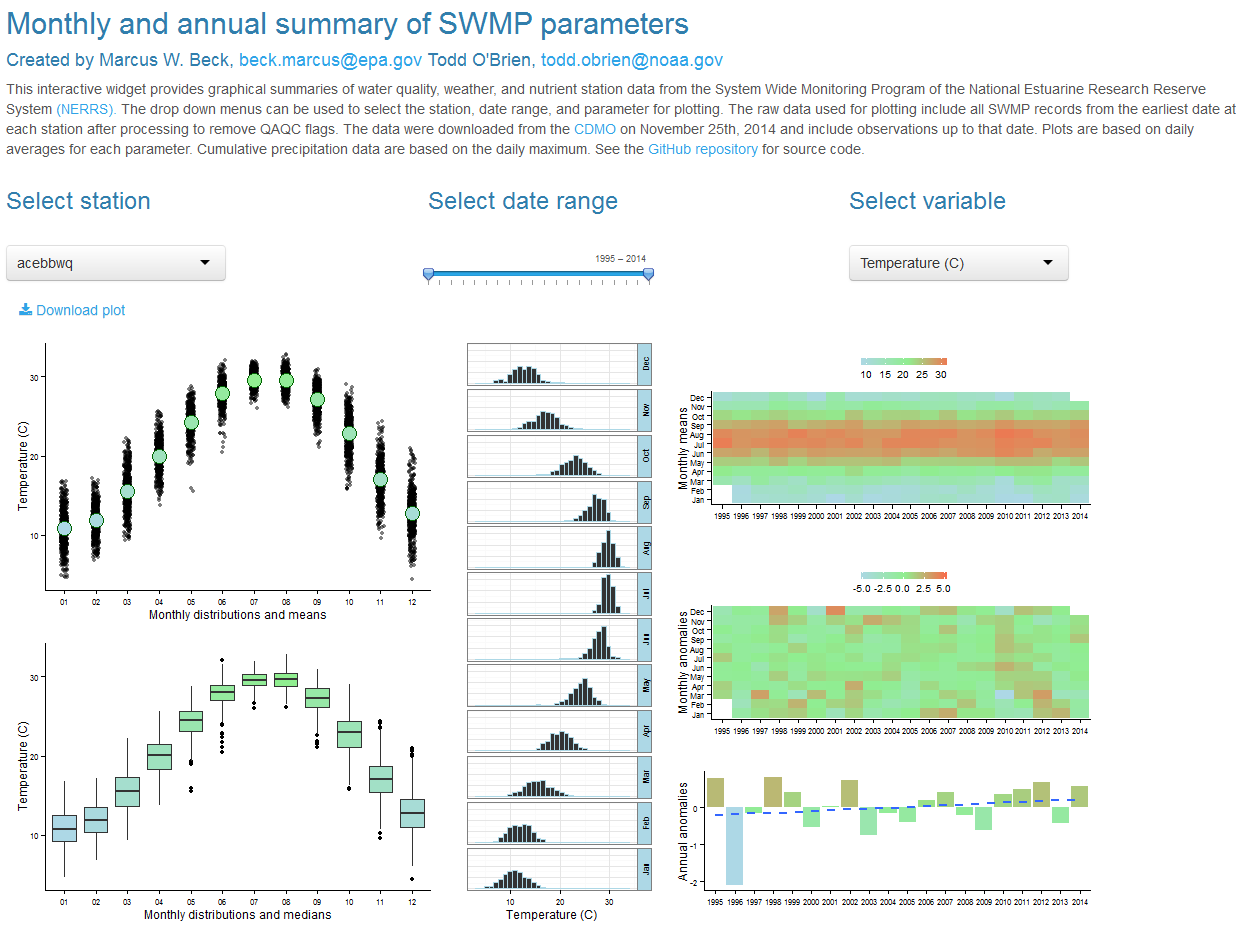
\includegraphics[width = 0.8\textwidth]{imgs/swmp_summary.png}}}
\end{frame}

%%%%%%
\begin{frame}{Widgets of SWMPrats.net: SWMP summary}
For a given \Bigtxt{site}, \Bigtxt{date range}, and \Bigtxt{variable}, it shows: \\~\\
\begin{itemize}
\item Monthly distribution with means (top left)
\item Monthly distributions by boxplots (bottom left)
\item Histogram frequency by month (center)
\item Monthly means by years (top right)
\item Monthly anomalies by year (center right)
\item Annual anomalies and trend (bottom right) \\~\\
\end{itemize}
Options for tabular data and saving plots/tables
\end{frame}

%%%%%%
\begin{frame}[fragile]{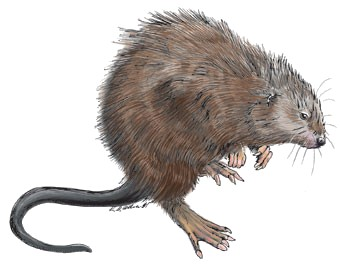
\includegraphics[width = 0.05\textwidth]{imgs/swmprat.png} Widgets of SWMPrats.net: SWMP summary}
Note: The \texttt{plot\_summary} function in SWMPr is used to create the plots.
\begin{knitrout}\scriptsize
\definecolor{shadecolor}{rgb}{0.969, 0.969, 0.969}\color{fgcolor}\begin{kframe}
\begin{alltt}
\hlkwd{library}\hlstd{(SWMPr)}

\hlcom{## import data}
\hlkwd{data}\hlstd{(apacpnut)}
\hlstd{dat} \hlkwb{<-} \hlkwd{qaqc}\hlstd{(apacpnut)}

\hlcom{## plot}
\hlkwd{plot_summary}\hlstd{(dat,} \hlkwc{param} \hlstd{=} \hlstr{'chla_n'}\hlstd{,} \hlkwc{years} \hlstd{=} \hlkwd{c}\hlstd{(}\hlnum{2007}\hlstd{,} \hlnum{2013}\hlstd{))}

\hlcom{## get individaul plots}
\hlstd{plots} \hlkwb{<-} \hlkwd{plot_summary}\hlstd{(dat,} \hlkwc{param} \hlstd{=} \hlstr{'chla_n'}\hlstd{,} \hlkwc{years} \hlstd{=} \hlkwd{c}\hlstd{(}\hlnum{2007}\hlstd{,} \hlnum{2013}\hlstd{),}
  \hlkwc{plt_sep} \hlstd{=} \hlnum{TRUE}\hlstd{)}

\hlstd{plots[[}\hlnum{1}\hlstd{]]} \hlcom{# top left}
\hlstd{plots[[}\hlnum{3}\hlstd{]]} \hlcom{# middle}
\hlstd{plots[[}\hlnum{6}\hlstd{]]} \hlcom{# bottom right}

\hlcom{## get summary data}
\hlkwd{plot_summary}\hlstd{(dat,} \hlkwc{param} \hlstd{=} \hlstr{'chla_n'}\hlstd{,} \hlkwc{year} \hlstd{=} \hlkwd{c}\hlstd{(}\hlnum{2007}\hlstd{,} \hlnum{2013}\hlstd{),} \hlkwc{sum_out} \hlstd{=} \hlnum{TRUE}\hlstd{)}
\end{alltt}
\end{kframe}
\end{knitrout}
\end{frame}

%%%%%%
\begin{frame}{Widgets of SWMPrats.net: SWMP compare}
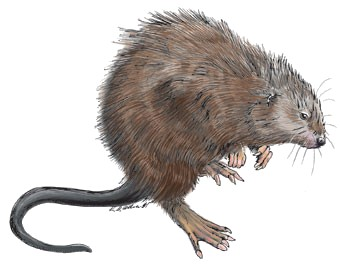
\includegraphics[width = 0.05\textwidth]{imgs/swmprat.png} Compare trends for a single parameter between reserves/space
\centerline{\fbox{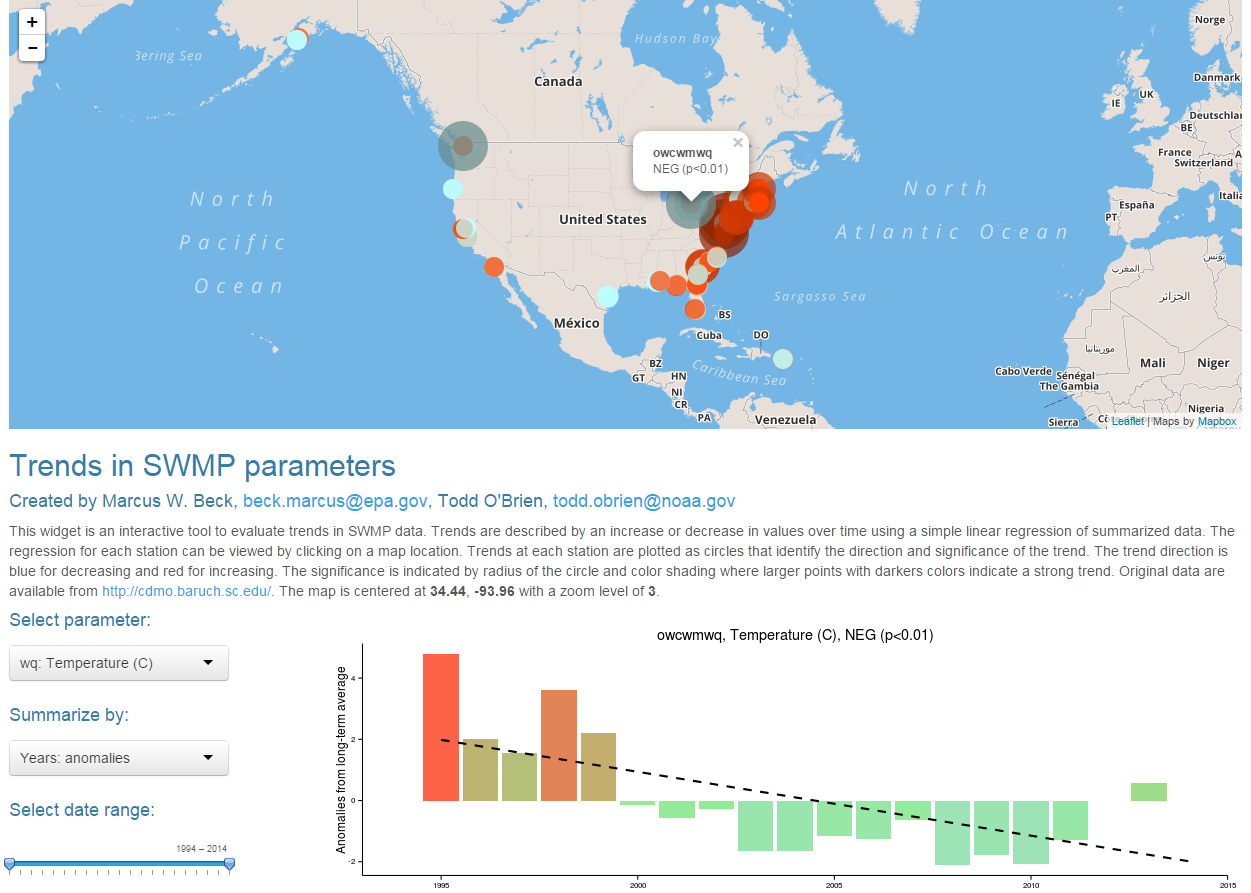
\includegraphics[width = 0.8\textwidth]{imgs/swmp_comp.png}}}
\end{frame}

%%%%%%
\begin{frame}{Widgets of SWMPrats.net: SWMP compare}
\onslide<1->
For a \Bigtxt{given parameter} and \Bigtxt{date range}, at all sites: \\~\\
\begin{itemize}
\onslide<1->
\item Evaluate annual or monthly changes\\~\\
\onslide<2->
\item Evaluate anomalies (difference from grand mean) or observed \\~\\
\onslide<3->
\item Trends shown as increasing (red), decreasing (blue) \\~\\
\onslide<4->
\item Significance (based on simple regression) is shown as size of point \\~\\
\end{itemize}
\onslide<5->
All trends are relative (\Bigtxt{compare})... \\~\\
Zoom the map to view finer spatial scale and click to view results for single stations
\end{frame}

%%%%%%
\begin{frame}{Widgets of SWMPrats.net: SWMP aggregate}
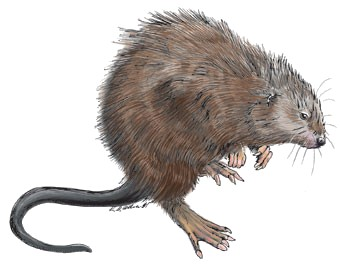
\includegraphics[width = 0.05\textwidth]{imgs/swmprat.png}  Compare aggregated parameters within and between reserves
\centerline{\fbox{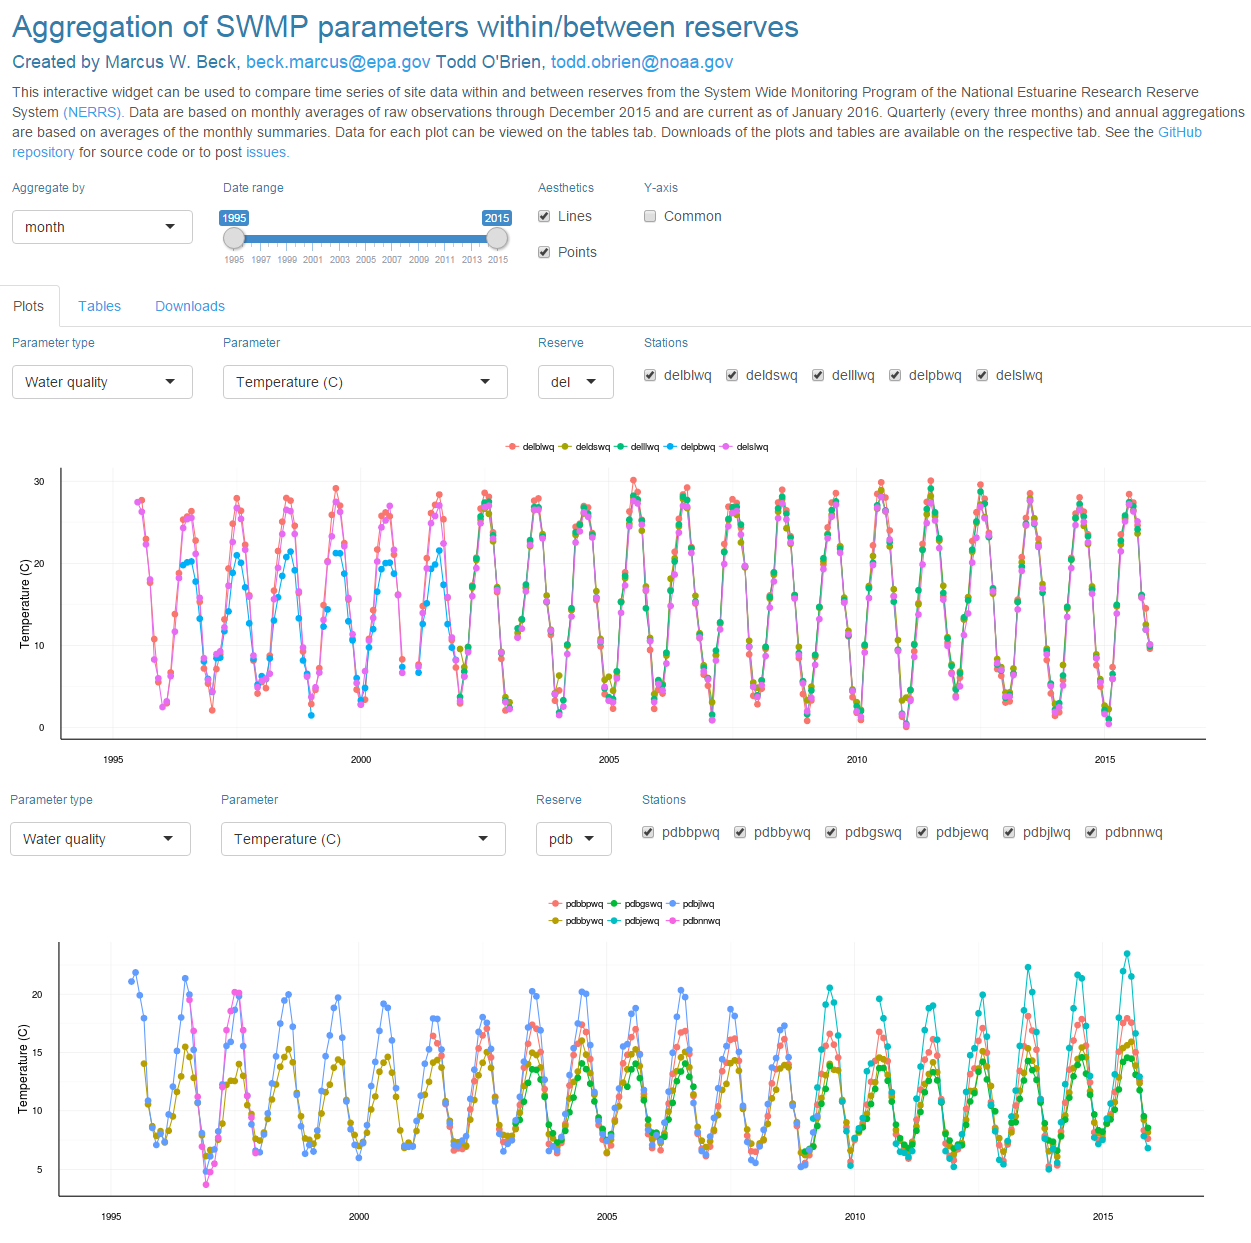
\includegraphics[width = 0.6\textwidth]{imgs/swmp_agg.png}}}
\end{frame}

%%%%%%
\begin{frame}{Widgets of SWMPrats.net: SWMP aggregate}
\onslide<1->
This app allows multiple comparisons: \\~\\
\begin{itemize}
\onslide<1->
\item Within and between sites \\~\\
\onslide<2->
\item Same or different parameters \\~\\
\onslide<3->
\item Seasonal (monthly, quarterly) or annual trends \\~\\
\onslide<4->
\item Options for tabular data and saving plots/tables \\~\\
\end{itemize}
\onslide<5->
Water and air temperature example at ACE basin.... note the common y-axis and effect of aggregating incomplete years
\end{frame}

%%%%%%
\begin{frame}
\vspace{0.3in}
\centerline{
\begin{tikzpicture}
  \node[drop shadow={shadow xshift=0ex,shadow yshift=0ex},fill=white,draw] at (0,0) {
\includegraphics[width=0.9\textwidth]{imgs/workshop2016logo.png}};
\end{tikzpicture}}
\vspace{0.5in}
\centerline{Up next... Time Series Topic 1: Weighted Regression}
\vspace{0.5in}
\Large
\centerline{\Bigtxt{Questions??}}
\end{frame}

\end{document}
